\documentclass[
paper=164mm:234mm,
pagesize,
DIV=calc,
10pt,
parskip=half-]{scrbook}

% --- CONFIGURATION ---
%-- Page Layout
\pagestyle{plain} % No header only footer
\interfootnotelinepenalty=10000 % do not split footnote across pages
\raggedbottom % allow whitespace at bottom of pages instead of streching parskip
\usepackage[a4, center, cam]{crop} % display crop marks


%-- Language and encoding
\usepackage[ngerman]{babel} % Required for "Neue Deutsche Rechtschreibung"
\usepackage[utf8]{inputenc} % Required for german umlauts
\usepackage[german=swiss]{csquotes} %Swiss quotation style << >>
\usepackage[T1]{fontenc} % Improves rendering of umlauts, quotes usw. in pdf


%-- Images and Caption
\usepackage{graphicx} % Required for including pictures
\usepackage{float} % Required for displaying images exactly where they appear in the source code
\usepackage[hypcap]{caption} % Required for image caption
\usepackage{wrapfig} % Allows in-line images
\graphicspath{{images/}} % Path to image folder
\usepackage{chngcntr} % FRequired for \counterwithout
\counterwithout{figure}{chapter} % figures without chapter number
\renewcommand{\figurename}{Abb.} % change caption identifier


%-- Citation, Bibliography
\usepackage[style=authoryear, backend=biber, bibwarn=true]{biblatex} % Bibliography style
\addbibresource{OpenSourceAndArt.bib} % Bibliography File
\setlength\bibitemsep{2mm} % Increased space between bibliography entries
\addto{\captionsngerman}{%
\renewcommand{\figurename}{Abb.} % Changes "Abbildung" in captions to "Abb."
}
\DefineBibliographyStrings{ngerman}{%
  bibliography = {Literaturverzeichnis} % Changes "Literatur" to "Literaturverzeichnis"
}


%-- Todo Markup
\usepackage{color, soul} % Required for highliting todo items
\newcommand{\comment}[1]{} % Allows multi line comments (http://tex.stackexchange.com/questions/44282/multiline-comment)
\newcommand{\todo}[1]{[\hl{TODO:} #1]} % For todo items


%-- Typography
\usepackage{lmodern} % Font Roboto Light
\usepackage[T1]{fontenc} % Improves rendering of umlauts, quotes usw. in pdf
\renewcommand{\familydefault}{\sfdefault}
\usepackage[protrusion=true,expansion=true]{microtype} % Better typography
\usepackage{hyperref} % Required for clickable hyperlinks
\linespread{1.05} % Change line spacing here, Palatino benefits from a slight increase by default
\renewcommand\UrlFont{\itshape} %Italic Hyperlinks





% --- DOCUMENT ---
\begin{document}

% --- TITLE ---
\extratitle{\null \vfill

\includegraphics[width=0.15\textwidth]{cc_by_sa} \\
\footnotesize{\emph{Open Source in den Digitalen Künsten} von Jonas Probst steht unter der Creative Commons Attribution-ShareAlike 4.0 International Lizenz. Die Weitergabe ist nur unter gleichen Bedingungen und mit Namensnennung möglich. Eine Kopie dieser Lizenz befindet sich unter \url{http://creativecommons.org/licenses/by-sa/4.0/}.\\

Diese Arbeit wurde in LaTeX verfasst, einer auf dem Textsatzsystem TeX beruhenden Auszeichnungssprache (engl. markup language). Der Quellcode befindet sich unter \url{http://github.com/jonasprobst/open-source-and-the-digital-arts}.}
}

\title{Open source in den Digitalen Künsten}
\author{Jonas Probst}
\date{\today}
\publishers{Hochschule der Künste Bern \\ MA Contemporary Arts Practice}


\lowertitleback{\normalsize{
Herzlichen Dank an:\\
Andi Schoon, Rikka Feuz, Roger Villars, Micha Haarenberg und Hansjürg Wenger.}}
%\dedication{}
\maketitle % Print the title section


% -- Table of content
\newpage
\thispagestyle{empty}
\tableofcontents

% -- ESSAY BODY ---
\phantomsection
\addcontentsline{toc}{chapter}{Einleitung}
\chapter*{Einleitung}
In meiner künstlerischen Praxis bin ich immer wieder mit dem Thema Open Source konfrontiert. Das Werk \emph{Color Permutations} (2012) nutzt ein Open Source Framework\footnote{Eine Liste der in der Einleitung erwähnten Open Source Projekte mit Weblinks findet sich im Anhang.} und läuft in einem Open Source Webbrowser auf einem Open Source Betriebssystem. Die \emph{Ewige Pfütze} (2013) wird von einem Open Source Mikrocontrollersystem gesteuert, für welches ich auf einer Open Source Programmierumgebung in einer dem Open Standard unterliegenden Programmiersprache\footnote{JavaScript ist ein ECMA-Standard \url{http://www.ecma-international.org/ecma-262/5.1/}. ECMA ist eine internationale Normungsorganisation zur Normung von Informations- und Kommunikationssystemen mit Sitz in Genf.} Algorithmen entwickelt habe.

Auch für mein nächstes Projekt werde ich von Open Source Hard- und Software Gebrauch machen. Denn damit stehen mir eine Vielzahl von ausgeklügelten Bausteinen zur Verfügung, die sich in anderen Projekten bereits mehrfach bewährt haben. Ähnlich einem Lego-Baukastensystem kann ich einzelne Teile zu einem System zusammenfügen, welches dann die technische Grundlage für die Umsetzung meiner Arbeit bildet. Die einzelnen Bausteine selbst zu entwickeln übersteigt meine Ressourcen, auch steht solch ein massgeschneidertes System nicht bei irgend einem Supermarkt im Regal. Dank den Open Source Technologien, kann ich meine Vision kostengünstig und effizient umsetzen, ohne das Rad neu erfinden zu müssen. Doch was ist Open Source (auf Deutsch offener Quellcode) eigentlich? Der Begriff stammt ursprünglich aus der Software Entwicklung und bedeutet dort in seiner Essenz, dass ein Autor freiwillig auf einen Teil seiner Urheberrechte verzichtet und den Quellcode seiner Software der Öffentlichkeit zugänglich macht. Diese Software kann sodann frei weiterverwendet, weiterentwickelt und den eigenen Bedürfnissen angepasst werden, ohne sich um Patent- oder Lizenzrechte sorgen zu müssen.

Was seit den neunziger Jahren die Computerwelt revolutioniert, zieht heute Kreise weit über Software hinaus. Da gibt es nebst den bereits erwähnten Projekten auch Strickautomaten, 3D-Drucker, Lexika, Handprothesen, humanoide Roboter, Video Games und Gamekonsolen. Dank Open Source CNC-Fräsmaschinen lassen sich Open Source Häuser mit Open Source Möbelstücken einrichten. Zur in Open Source Zeichensätzen dargestellten Open Source Sciencefiction-Novelle geniesst der Kenner ein Open Source Bier. Und wo es Freibier gibt, ist auch Kultur zu finden: Pop-Musik, Comic Strips, Animationsfilme, Spielfilme sogar ein Filmfestival und eine Open Source Galerie.


Der Hype hat auch die bildende Kunst erreicht. Besonders bei den \emph{Digitalen Künsten}\footnote{Ein von Cat Hope und John Ryan geprägter Überbegriff der Kunstformen  New Media Art, Electronic Art, Computer Art, Internet Art, Post Media Art, Telematic Art, Virtual Art usw. Siehe \cite[3-12]{Hope-Ryan:2014}.}, wenn Software oder Elektronik ins Spiel kommt, ist Open Source nicht weit. Sei es im Theater, Tanz oder in der Performance, der elektronischen Musik, Internetkunst oder wie in meinem Beispiel der Installation. Doch jedes Mal, wenn ich zur Umsetzung einer Arbeit auf Open Source setze, sehe ich mich mit den gleichen Fragen konfrontiert. Was bedeutet Open Source für die Kunst? Für meine Kunst? Für meine Autorschaft? Wie stehe ich dazu, wie gehe ich damit um?
Eine ganze Armee von Individuen kollaboriert, meist unbezahlt und in der Freizeit, übers Internet an Projekten, ohne die ich meine Kunstwerke nicht realisieren könnte. Nutze ich das schamlos aus oder gebe ich etwas zurück? In welcher Form könnte ich als Künstler in diesem Umfeld überhaupt mitwirken?

Dann ist da noch die sogenannte \emph{Share Alike} Klausel, auch \emph{Copyleft} genannt. Weil ein Autor seine Urheberrechte explizit abgeben muss, stehen alle Open Source Projekte unter einer Open Source Lizenz.\footnote{Eine Übersicht der von der Open Source Foundation anerkannten Lizenzen findet sich auf \url{http://opensource.org/licenses} (12.02.2015).} Natürlich ist jeder Autor frei, für welche Geschmacksrichtung er sich entscheidet: Ob er zum Beispiel alle Urheberrechte abtritt, eine kommerzielle Nutzung ausschliesst oder eben vorgibt, dass alle Bearbeitungen unter gleichen Bedingungen weitergegeben werden müssen.\footnote{Die Creative Commons \url{http://creativecommons.org} (12.02.2015) bietet eine Alternative zum Copyright an. Ein modulares Lizenzsystem, welches eine feinere Abstufung des \enquote{Alle Rechte Vorbehalten} zulässt. Siehe \cite[7-8]{Casserly-Ito:2011}.} Der Konsequenz des Letzteren sind sich wohl die wenigsten Künstler bewusst, die von Open Source Gebrauch machen. Denn wenn ich demnach Ressourcen nutze, die einer \emph{Share Alike} Lizenz unterstehen, verpflichte ich mich dazu, mein darauf aufbauendes Werk wiederum unter derselben Lizenz der Öffentlichkeit zu überlassen.

Welche Auswirkungen hat ein solches Vorgehen auf den Kunstmarkt? Beschränkt sich das Prinzip von Open Source in der Kunst lediglich auf die Technik zur Herstellung oder findet es darüber hinaus Anwendung? Wenn ja, was wäre dann der Quellcode der Kunst, der offengelegt werden müsste?

Das Phänomen Open Source hat viele Seiten und diverse Schnittpunkte mit anderen Wissenschaften - dieses Thema umfassend abzuhandeln, übersteigt diese Arbeit bei weitem. Deshalb setze ich den Schwerpunkt einer ersten Annäherung bei der Frage, wie andere zeitgenössische Künstler mit dem Thema Open Source umgehen. Zuerst leite ich aus der Entstehungsgeschichte von Open Source einige Kern- und Kennwerte ab, um darauffolgend die !Mediengruppe Bitnik und Christian Waldvogel am Beispiel der gemeinsamen Ausstellung im Helmhaus Zürich\footnote{Christian Waldvogel, \emph{unknown} (\cite{Waldvogel:2014}) und Mediengruppe Bitnik, \emph{Delivery for Mr. Assange} (\cite{Ryser/MediengruppeBitnik:2014}) im Helmahus Zürich 14.02. - 06.04.2014.} zu untersuche. Schliesslich entwickle ich aus diesen Erkenntnissen einen Prototyp für den Umgang mit Open Source in meiner eigenen künstlerischen Praxis.


% ---
\phantomsection
\addcontentsline{toc}{chapter}{Was ist Open Source?}
\chapter*{Was ist Open Source?}

Der Begriff \emph{Open Source} stammt aus der Softwareentwicklung und heisst soviel wie \enquote{offener Quellcode}. Der Quellcode beschreibt den Ablauf eines Programms in einer für Menschen lesbaren Form. Meist ist dies ein strukturierter Text im Syntax einer Programmiersprache. Allerdings kann ein Computer mit dem Quellcode nicht viel anfangen. Damit er solche Programme ausführen kann, müssen sie in maschinenlesbare Sprache übersetzt, sprich kompiliert werden.

Aus der resultierenden Struktur von Einsen und Nullen ist es gänzlich unmöglich, den ursprünglichen Quellcode zu rekonstruieren. Viele Softwarehersteller veröffentlichen deshalb ihre Programme ausschliesslich in kompilierter Form als Binärdateien, den Executables. Auf diese Weise kann so genannte proprietäre Software als Produkt vermarktet werden.

Was uns heute selbstverständlich scheint, war nicht immer so: \enquote{In den frühen Tagen des Computers war alle Software quelloffen und frei.}\footnote{\cite[202]{Grassmuck:2004}.}.


\phantomsection
\addcontentsline{toc}{section}{Ursprung des offenen Quellcodes}
\section*{Ursprung des offenen Quellcodes}

Anfänglich bestand für Software kein eigenständiger Markt. Sie war kostenlose Zugabe zur Hardware oder wurde von ihren Nutzern gleich selbst geschrieben. Quellcode zirkulierte frei, Programme wurden laufend verbessert, weiterentwickelt und die Ergebnisse an die Nutzergemeinschaft zurück gegeben.

Erst in den 70er Jahren, so schildert es der Medienwissenschaftler Volker Grassmuck, zeichnete sich eine Trendwende ab. Unter dem Druck des vom US-Justizministerium eingeleiteten Kartellverfahrens gab IBM die Bündelung von Hardware mit Software, Peripheriegeräten, Wartung und Schulung auf. Diese Entkopplung schuf die Voraussetzungen für eine eigenständige Softwareindustrie - Software wurde erstmals zur Ware\footnote{\cite[203]{Grassmuck:2004}.}.

Die darauffolgende vollständige Kommerzialisierung von Software hängt für Grassmuck mit der Erfolgsgeschichte von Microsoft (gegründet 1975) zusammen. Diese begann mit dem Betriebssystem DOS, das Microsoft nicht selber entwickelt, sondern von einer anderen Firma aufgekauft hatte. Als IBM in den 80er Jahren ein Betriebssystem für den ersten Personal Computer suchte, fiel der Entscheid eher durch Zufall\footnote{Das weiter verbreitete und bessere Betriebssystem für die damalige Generation von 8-Bit-Rechner war CP/M (Control Program for Microcomputers), das Gary Kildall entwickelt hatte. \enquote{Das Millionengeschäft mit IBM ging jedoch an Microsoft, das damals vor allem für das auf fast jedem Mikrocomputer verfügbare MS-BASIC bekannt war, weil Kildall einer Anekdote nach am entscheidenden Tag mit seinem Privatflugzeug unterwegs und damit nicht erreichbar war.} \cite[205]{Grassmuck:2004}.} auf DOS. Doch sicherte sich Microsoft dank der schnellen Verbreitung des PCs innerhalb von kurzer Zeit ein Monopol, das es mit der grafischen Benutzeroberfläche Windows und zahlreichen weiteren Anwendungen konsequent ausbaute. Dabei setzte es auf eine Strategie des „Bundling“: Die verschiedenen Microsoft-Programme bauen so aufeinander auf, dass sie schwer durch andere Software ersetzt werden können. Weil sie nur in kompilierter Form erscheinen, können sie nicht angepasst und weiterentwickelt werden. Auf diese Weise, so schliesst Grassmuck, machte Microsoft nicht nur seine Produkte, sondern auch sein System der kommerziellen Verwertung zum allgemeinen Standard: \enquote{Anfang der 80er war fast alle Software proprietär}.\footnote{\cite[221]{Grassmuck:2004}.}

Natürlich sträubten sich viele Urväter von Software gegen das auferlegte kommerzielle Korsett, das Copyright, den geschlossenen Quellcode und kommunikationswidrige Vertraulichkeitsvereinbarungen.\footnote{Diese auf engl. \emph{Nondisclosure Agreements} verboten es explizit, Code frei anzupassen und untereinander auszutauschen.} Der populärste Aufständische ist der exzentrische Software Freedom Aktivist und Programmierer Richard Stallman,\footnote{Die Webseite von Stallman bietet Einblick in sein vielseitiges politischen Engagement und weit über Software hinaus auch in sein intimstes Privatleben. Siehe \url{https://stallman.org/} (17.12.2014).} der 1984 seinen Job am Massachusetts Institute of Technology (MIT) kündigte, um ein Betriebssystem zu entwickeln, das wieder frei sein sollte. Denn nur wenn das Betriebssystem selbst - der Kern des Computers der alle anderen Programme ausführt - \emph{alle} Software-Freiheitsrechte einhält, kann es sie dem Anwender gewähren.\footnote{\cite[9]{Stallman:2010}.}

Sein neues Betriebssystem sollte auf dem beliebten und weitverbreiteten \emph{Unix} basieren. Dieses stammte aus der Zeit, in der Software noch frei war, doch wurde es vom amerikanischen Telekommunikations-Konzern AT\&T allmählich kommerzialisiert. Der Plan war, Zeile um Zeile jedes einzelnen Teils des privatisierten Codes von Unix zu ersetzen. Stallman nutzte dazu die beginnende Vernetzung von Forschungseinrichtungen, Universitäten und Unternehmen über das Internet. Sein Projekt stellte er in Newsgroups vor und lud zur Mitarbeit ein. Der erste Coup, ein hocheffizienter C-Compiler \emph{GCC} und ein sehr flexibler und anpassbarer Text Editor \emph{Emacs}, stiess auf grosse Resonanz. Schnell fanden sich Gleichgesinnte und schliesslich wurde zur Verbreitung der Programme und ihrer Ideologie die \emph{Free Software Foundation} gegründet.\footnote{\cite[7-25]{Stallman:2010}; Vgl. auch \cite[217-227]{Grassmuck:2004} und \cite[18-19]{Raymond:1999}.}

Nun durften diese Programme keinesfalls das gleiche Schicksal treffen wie vormals Unix. Deshalb schrieb Stallman 1989 die erste Lizenz für freie Software, die \emph{GNU General Public License} (GPL).\footnote{Die aktuellste Version ist die GNU GPL v3 \url{https://www.gnu.org/licenses/} (18.12.2014). Für ältere Versionen siehe \url{https://www.gnu.org/licenses/old-licenses/old-licenses.html} (18.12.2014).} Anders als das Copyright schützt sie nicht den Rechteinhaber, sondern die Freiheit der Software selbst. Die GPL definiert vier Freiheiten, die dieses Prinzip des Copyleft gewährleisten: Ein Programm gilt nur dann als freie Software, wenn (1) sein Quellcode offen zugänglich ist, wenn (2) es kopiert und weitergegeben werden darf, wenn (3) Veränderungen vorgenommen und diese (4) wiederum weitergegeben werden dürfen.\footnote{Siehe \emph{GNU Free Software Definition} \cite[3]{Stallman:2010}.}

Auf der Grundlage der vier Freiheiten wurde das GNU-System kontinuierlich weiter entwickelt. 1990 fehlte nur noch der Kernel, die zentrale Verbindung zwischen Software und Hardware. Diese Aufgabe nahm der finnische Informatikstudenten Linus Torvalds in Angriff. Bereits sehr früh veröffentlichte er das unfertige Programm im Internet und rief zur Kollaboration auf.\footnote{Siehe dazu \cite{Torvalds:1999}.} Aus allen Teilen der Welt meldeten sich Freiwillige, die bereit waren, Arbeit und Zeit ohne Bezahlung in ein gemeinsames Projekt zu investieren. Änderungen und Verbesserungen am Quellcode wurden von Torvalds unverzüglich eingearbeitet und auch täglich neu veröffentlicht. Torvald glänzte dabei nicht selbst als Entwickler, sondern vorallem als Organisator und Motivator. Und so kam es, dass wieder Erwarten Tausende von Menschen in einer verteilten, offenen, locker gekoppelten Zusammenarbeit das komplexe Softwareprojekt Linux entwickelten.\footnote{Siehe \cite{Raymond:2001}; Vgl. auch \cite[227]{Grassmuck:2004}.}

Mit dem Erfolg von Linux etablierte sich das Prinzip des offenen Quellcodes. Das kollaborative Entwicklungsmodell komplettierte das \enquote{Open Source Dreieck aus Technik, Recht und neuen Kooperationsformen}\footnote{\cite{Deterding:2007}.} und gewann rasch an Bedeutung. Zur Überraschung aller Free Software Enthusiasten entschied Netscape 1998, als erster proprietärer Softwarehersteller überhaupt, den Quellcode ihres gleichnamigen Internetbrowsers\footnote{Heute bekannt unter dem Namen Mozilla Firefox \url{http://www.mozilla.org}. Mozilla wurde von Netscape gegründet, um unter einem neutralen Namen den Quellcode zu veröffentlichen und die Entwicklergemeinschaft zu pflegen \cite[91]{Hamerly-Paquin-Walton:1999}} unter einer Open Source Lizenz öffentlich zugänglich zu machen. Um weitere Unternehmen für die Sache zu gewinnen, wurde im selben Jahr die Open Source Initiative\footnote{Siehe dazu \url{http://opensource.org/}.} um den Programmierer Eric Raymond gegründet. Zudem wurden neue liberalere Lizenzen\footnote{Die GNU GPL Lizenz ist viral. Werden Programmteile die unter dieser Lizenz stehen mit anderen kompiliert, unterliegt das Endprodukt und somit der gesamte Quellcode der GPL. Die GPL ist demnach nicht kompatibel mit anderen Lizenzformen und verhindert so gezielt, nur Teile eines Programms quelloffen zu machen und die Anderen \enquote{geschlossen} zu verkaufen. Siehe \cite[93]{Hamerly-Paquin-Walton:1999}.} geschaffen, die speziell auf Unternehmen zugeschnitten waren. Der neue Name \emph{Open Source Software} (OSS) verbreitete sich schnell, sorgte aber bald für Konflikte. Für Anhänger der alten Bezeichnung \emph{Free Software} verkürzte er das umfassende Prinzip der Freiheit einer Software auf das technische Kriterium des offenen Quellcodes. In der Bezeichnung \emph{FOSS} (Free and Open Source Software) beziehungsweise \emph{FLOSS} (Free/Libre and Open Source Software) wurde ein Kompromiss gefunden, der sich aber bisher noch nicht richtig durchgesetzt hat.

Ungeachtet der Bezeichnung, steht Open Source für ein Konzept, dessen Erfolg mittlerweile kaum zu übersehen ist: Nebst einer Vielfalt von Code-Bausteinen, sogenannten Frameworks und Libraries, laufen Linux basierte Betriebssysteme auf vielen Firmen-Servern, Privat-Computern und Smartphones. Googles Chromium und Mozillas Firefox sind die am weitesten verbreiteten Webbrowser im Netz\footnote{Gemäss dem Internet Statistik Dienst w3counter.com (\url{http://www.w3counter.com/globalstats.php}) sind zur Zeit Chrome (42.7\%) gefolgt von Firefox (16.4\%) vor Internet Explorer (15.8\%) die meist genutzten Webbrowser.} und Programme wie OpenOffice, Gimp, Thunderbird, VLC und Wordpress sind aus dem Alltag kaum mehr wegzudenken. Sogar bei Microsoft zeichnet sich ein Umdenken ab, im Herbst 2014 startete Microsoft den Openness Blog\footnote{Siehe \url{http://openness.microsoft.com/blog/}; Vgl. auch \url{http://www.microsoft.com/en-us/openness}.} und veröffentlichte den Quellcode für die Web-Entwicklungsplattform DotNet.\footnote{Der Quellcode kann unter \url{https://github.com/Microsoft/dotnet)} eingesehen werden.}

Open Source ist also mehr als nur ein Hype, wie die stetig wachsenden Marktanteile quelloffener Software eindrücklich belegt. Doch warum ist das Phänomen so erfolgreich? Warum setzt eine wachsende Anzahl von Firmen und Regierungen\footnote{Sogar die Europäische Union hat eine Strategie für Open Source Software. Siehe \emph{Strategy for internal use of OSS at the EC} unter \url{http://ec.europa.eu/dgs/informatics/oss_tech/index_en.htm} (24.12.2014).} auf Open Source? Und was treibt einen Software-Entwickler dazu, in seiner Freizeit Software zu schreiben nur um sie anschliessend zu verschenken?


\phantomsection
\addcontentsline{toc}{section}{Hackerethik und der Geist der Quelloffenheit}
\section*{Hackerethik und der Geist der Quelloffenheit}

Die Computer Enthusiasten des MIT Modelleisenbahn Clubs (MIT Tech Model Railroad Club) nannten sich selber Hacker, nach der Aktivität der Programmierer, die auf der Computertastatur herum hacken (auf englisch hacking).\footnote{\cite[10]{Levy:1984}.} Dieser Namen beschreibt eine Gruppe von Menschen, die aus der seit 1945 heranwachsenden Computerkultur hervorging. Die vorwiegend aus jugendlichen Studierenden und Universitätsangestellten bestehende Gruppe hatte ihre eigene fachspezifische Sprache,\footnote{Siehe Jargon File, das Kompendium der Hacker-Ausdrucksweise \url{http://www.catb.org/jargon/} (30.01.2015).} eigene Insider Witze\footnote{Zum Beispiel die Hacker Bibel: \emph{The Gospel According to Tux} siehe \url{http://www.armoredpenguin.com/~regan/penguins/tux.html} (30.01.2015). Tux ist der Name des Linux Pinguin-Maskottchens.} und Dresscodes.\footnote{Für einen Einblick in die Hackerkultur siehe \cite[16]{Raymond:1999}; Vgl. auch \cite{Raymond:1996}.}

Hacker waren vom Computer fasziniert - Programmieren war das Mittel zur Erkundung seiner Möglichkeiten. Motiviert, nicht aus finanziellen Interessen sondern aus blosser Wissbegierde, wagten sie abenteuerliche Entdeckungsreisen in die neue Welt dieser Maschinen. Vermutlich dank ihrer wissenschaftlichen Prägung war es für sie selbstverständlich, ihre Forschungsergebnisse zu publizieren und sie anderen zur Examination und freien Weiterverwendung zu unterbreiten. So wurde Software gratis, frei und bedenkenlos unter den verschiedenen Forschungszentren ausgetauscht,\footnote{So auch \emph{Spacewar!} eines der ersten Computer Spiele überhaupt und Relikt der Hackerkultur. Es wurde 1961 am MIT von Steven Russel für den DPD-1 entwickelt und verbreitete sich schnell in andere Forschungszentren, wo es ergänzt und weiterentwickelt wurde.} und es herrschte ein heiteres Klima des offenen Miteinanders.

Der hier beschriebene Typ von Hackern ist nicht zu verwechseln mit \enquote{Computer Kriminellen}, wie man sie aus den Medien im Zusammenhang mit Computersicherheit kennt. Die Ersteren waren Computer Liebhaber und Programmierer aus Leidenschaft, mit einem Ehrenkodex, der unterschiedlicher nicht sein könnte.

Der Reporter Steven Levy versuchte als Erster die neue computerzentrierte Subkultur zu beschreiben. Unter dem Begriff \emph{Hacker Ethik} leitete er daraus die nachfolgende sechs Kernwerte ab.
(1) Der Zugang zu Computern und allem, was uns Erkenntnis über die Funktionsweise der Welt bringen könnte soll grenzenlos und total sein. Nur wenn ein Hacker uneingeschränkten Zugang hat, kann er von bereits existierenden Ideen und Systemen lernen, um diese weiter zu entwickeln und zu verbessern. Diesen Drang zur Verbesserung sieht Levy indes als zentrales Kennzeichen eines Hackers, den sogenannten \emph{Hands-On Imperative}: Programmierer sind darauf getrimmt, Programme in ihre Einzelteile zu zerlegen, sie zu analysieren und auf diesen Erkenntnissen aufbauend den Algorithmus zu verbessern oder neu zu erfinden. Dieses Prinzip weiten Hacker auf alle anderen Bereiche ihres Lebens aus.
(2) Alle Information soll frei sein. Aufbauend auf dem Prinzip des Zugangs muss Information auch frei von Einschränkungen sein, damit ein Hacker das System verbessern kann.
(3) Autorität soll misstraut werden, Dezentralisierung ist zu bevorzugen. Nur eine flache Hierarchie in einem offenen System bietet dem Hacker die oben genannten Freiheiten. Jegliche Art von Bürokratie erschwert seine Arbeit.
(4) Hacker sollen nur nach ihrer Fähigkeit zu hacken beurteilt werden, nicht nach Kriterien wie Rasse, Klasse, Alter oder Stellung. Die Hacker sind leistungsorientiert, in Anbetracht ihres Könnens sind genannte Kriterien unwichtig.
(5) Computer können benutzt werden, um Kunst und Schönes zu schaffen. Für einen Hacker kann ein durchdachtes, effizientes und schön arrangiertes Programm durchaus ein Kunstwerk sein, denn schliesslich sind dies Qualitätsmerkmale für Quellcode.
(6) Computer können das Leben zum Besseren wenden. Ein Hacker sind so begeistert von der unbegrenzten Welt der Computer, dass er Andere daran teilhaben lassen möchte.\footnote{Siehe \cite[26-37]{Levy:1984}.}

Die beschriebene \emph{Hacker Ethik} ist stark mit der damaligen Situation der Hacker am MIT verstrickt. Zum Beispiel mussten die Studenten die zur Verfügung stehende Zeit am einzigen Computer im Institut untereinander teilen. Gleichzeitig verstanden sich die Hacker aber als Vorreiter eines neuen Technologiezeitalters und meinten es mit diesen Kernwerten, auch über die Universitätsgrenzen hinaus, durchaus ernst.\footnote{\cite[26]{Levy:1984}.}

Der finnische Philosoph und Computerwissenschaftler Pekka Himanen definierte 2001 den mittlerweile weit verbreiteten Begriff der Hackerethik in seinem gleichnamigen Buch etwas allgemeiner. Für ihn ist ein Hacker jemand, der seiner Leidenschaft folgt und dabei Gutes für alle schafft.\footnote{\cite[3-6]{Himanen:2001}. Der australische Medienwissenschaftler McKenzie Wark vertritt in \emph{A Hacker Manifesto} eine ähnliche Sicht wie Himanen, seiner Ansicht nach ist alles und in allem Code. Der Hacker abstrahiert diese Datenfülle und schafft daraus neues, sei es in der Mathematik, Musik, Kunst usw. Siehe \cite[13]{McKenzie:2006}.} Himanen sieht darin eine neue Arbeitsethik, welche die protestantische in Frage stellt. Statt der von der protestantischen Arbeitsethik betonten Kontrolle, steht bei der Hackerethik Austausch und Freiheit im Vordergrund, die zu Wohlstand für alle führen soll. Der Hacker Codex, so Himanen, ähnelt dem Idealbild der Wissenschaft, einer wissenschaftlichen Gemeinschaft nach platonischem Vorbild.\footnote{\cite[7-19]{Himanen:2001}.} Das Höchste jedoch, da sind sich Himanen und Levy einig, ist die Kreativität. Der Hacker-Meister lebt nicht nur nach den Prinzipien der Hackerethik, sondern beweist sein Geschick durch innovatives, einfallsreiches und ausgereiftes (Programmier-)Kunsthandwerk.\footnote{\cite[141]{Himanen:2001}.}

Zusammengefasst ist die Hackerethik also eine Gesinnung des freiwilligen und selbst gewählten Arbeitens, der Kooperation und des Teilens über alle Grenzen hinweg, der radikalen Offenheit und Transparenz aller Informationen und der Freiheit, all diese Werte selbstbestimmt auszuleben mit dem Ziel, zu einer besseren Welt beizutragen.

Mit diesem stolzen Ziel voller Idealismus und waghalsigem Optimismus, gründete der \enquote{letzte wahre Hacker}\footnote{\cite[419]{Levy:1984}.} Richard Stallman 1985 die Free Software Foundation und startete damit die Open Source Bewegung - überraschenderweise mit grossem Erfolg.


\phantomsection
\addcontentsline{toc}{section}{Mit Offenheit Geschäfte machen}
\section*{Mit Offenheit Geschäfte machen}

Ein puristisches Open Source Projekt hat keine finanziellen Absichten. Es ist weder Resultat einer Marktstudie, noch geht es aus einem gross angelegten Start-Up hervor. Es entstehen vielmehr aus einem kollektiven Bedürfnis heraus, dort wo ein Mutiger einen ersten Schritt wagt.

\enquote{Ein Programmierer kratzt sich dort wo es ihn juckt}:\footnote{\cite[4]{Raymond:2001}.} Zum Beispiel, wenn ein Drucker Treiber nicht funktioniert wie erwartet. Der Legende nach hat sich Stallman dermassen über den vergeblichen Gang zum Drucker geärgert, das er kurzentschlossen einen eigenen Druckertreiber schrieb, welcher über den Status des Druckvorganges informierte.\footnote{\cite[32]{Raymond:1999}; Vgl. auch \cite[9]{Stallman:2010}.} Im Dickicht des Internets entstehen täglich unzählige ähnliche Projekte, da jederman ein Projekt starten kann. Entscheidend ist letztlich nur die Relevanz der Aufgabenstellung und der Nutzen für die Gemeinschaft (Community), denn nur einschlägige Projekte werden genug Aufmerksamkeit auf sich ziehen, um weitere Programmierer dazu zu bewegen, sich in das Projekt zu investieren.

Das ausschlaggebende Qualitätsmerkmal von Open Source Projekten ist nebst der Verbreitung die Grösse der Community. Denn nur wenn genügend Mitglieder die Sache vorantreiben, ist ein Weiterbestehen garantiert. Überhaupt ist Kollaboration der zentrale Aspekt, da das Schreiben von Software eine komplexe und zeitaufwendige Arbeit ist. Computer sind grundsätzlich dumm. Das Einzige worin sie brillieren, ist das Ausführen von immer gleichen Arbeitsschritten - dies hingegen tun sie in einer ungeheuren Geschwindigkeit. Somit ist es die Aufgabe des Software Entwicklers, eine vielschichtige Aufgabenstellung zu abstrahieren und in zig einfache Arbeitsschritte zu unterteilen. Diese müssen anschliessend möglichst detailliert beschrieben werden, damit ein Computer sie ausführen kann. Beide Arbeitsschritte, die Abstrahierung sowie das Niederschreiben, lassen sich im Team viel effizienter erledigen als im Einzelgang. Während dem Schreiben solcher Instruktionen schleichen sich gerne kleine Denk- und Schreibfehler ein, sogenannte \emph{Bugs},\footnote{Die Bezeichnung \emph{Bug} (deutsch Käfer) für Softwarefehler und \emph{Debugging} für deren Suche und Behebung, stammt der Legende nach von der Computerwissenschaftlerin Grace Hopper (1906-1992). Als Mitarbeiter an der Harvard Universität um 1940 als Ursache für einen Systemfehler des \emph{Mark II} Computers, eine in einem Relais feststeckende Motte fand, soll Hopper dies als \enquote{debugging} bezeichnet haben.} die das Programm zum Abstürzen bringen können. Auch da gilt, je mehr geschulte Augenpaare den Programmtext überprüfen, umso mehr Fehler können frühzeitig erkannt und behoben werden. Und nistet sich trotzdem ein Bug ein, so werden ihn tausend Kammerjäger schneller finden als ein einziger.\footnote{\cite[235-254]{Grassmuck:2004}.}

Gerade deshalb ist Open Source für Softwarefirmen ein interessantes Modell, denn viele Kundenprojekte kommen mit ähnlichen Aufgabenstellungen. Wer also geschickt arbeitet, isoliert einzelne Bausteine und kann diese dann immer wieder einsetzen. Proprietäre Softwarehersteller entwickeln ihre eigenen Code-Bausteine hinter verschlossenen Türen. Das führt immer wieder dazu, dass mehrere Unternehmen gleichzeitig ein fast identisches Produkt erfinden. Ein solches Vorgehen ist träge, teuer und unnötig aufwändig. Open Source bietet dazu eine einfache Alternative; die Zusammenarbeit. In neutralen Projekten entwickeln die verschiedenen Interessenten gemeinsam mit der Konkurrenz die Softwaregrundlage der Produkte. Dies spart personelle Ressourcen, erleichtert die Fehlerbehebung und garantiert eine innovative Weiterentwicklung. Verkauft wird nicht mehr die Software selbst, sondern Dienstleistungen darum herum wie IT-Beratungen, kundenspezifische Anpassungen oder der Unterhalt von Infrastrukturen.\footnote{\cite[329-357]{Grassmuck:2004}.}

Eine solche Kollaboration funktioniert nur, wenn alle Parteien gleichgestellt sind: Alle haben das gleiche Mitspracherecht und uneingeschränkten Zugriff auf den Quellcode. Dieser kann nach Belieben verändert, kopiert und weiterverbreitet werden. Dazu muss jeder auf die Urheberrechte seines Beitrages verzichten, im Wissen darum, dass der Mehrwert in der Zusammenarbeit liegt. Deshalb braucht es einen Vertrag, der nicht den Urheber, sondern die Freiheit und Offenheit des Quellcodes schützt - die Open Source Lizenz.


% ---
\phantomsection
\addcontentsline{toc}{chapter}{Open Source in der Digitalen Kunst}
\chapter*{Open Source in der Digitalen Kunst}

Die \emph{Digitalen Künste} haben ihre Wurzeln im frühen 20. Jahrhundert. Dadaismus, Fluxus, Konzeptkunst und Kunst im öffentlichen Raum haben neue Formen von Performance, Theater und Installation hervorgebracht. Sie erkundeten Konzepte, Prozesse, Happenings und Interaktion statt der traditionellen Materie-basierten Kunstformen. Auch die Avantgarde-Strömungen Konstruktivismus, Futurismus und Bauhaus haben mit ihrer Faszination für Technik und Maschinen-Ästhetik einen Beitrag geleistet.\footnote{\cite[39]{Hope-Ryan:2014}; Vgl. auch \cite{Taylor:2014}.} Schliesslich waren es jedoch Ingenieure, die um 1950 als Erste begannen, Elektronik für künstlerische Zwecke einzusetzen, allen voran Ben Laposky (1914 - 2000) mit seinen abstrakten Oszilloskop-Bildern \emph{Oscillons} (1953). Und nur wenig später folgte Michael Noll (*1939) mit seinen computergenerierten Zeichnungen wie \emph{Vertical-Horizontal No. 3} (1964). Er war Forscher an den \emph{Bell Labs} in Murray Hill New Jersey, dem Geburtsort von Transistoren, Laser und dem Betriebssystem UNIX.\footnote{\cite[24]{Wands:2006}.}

Die aufkeimende Zusammenarbeit von Kunst mit Natur- und Ingenieurswissenschaften der sechziger Jahre wurde von Organisationen wie \emph{Experiments in Art and Technology} (E.A.T.)\footnote{E.A.T. wurde 1967 von den Ingenieuren Billy Klüver und Fred Waldhauer sowie den Künstlern Robert Rauschenberg und Robert Whitman gegründet. Ihr Ziel war die Förderung der Kollaboration von Künstlern mit Ingenieuren, indem sie ein Netzwerk zum Knüpfen von Kontakten aufbauten. Siehe \cite[16]{Paul:2003}.} weiter gefördert. Immer mehr Künstler begannen sich der neusten Technik zu bedienen, und so mündete das interdisziplinäre Miteinander in Nam June's Video Kunst \emph{Participation TV} (1963), in Installationen wie \emph{Legible City} (1988) von Jeffrey Shaws (*1944) und Performances wie \emph{Ping Body} (1996) von Stelarc (*1946).\footnote{\cite[96]{Graham:2007}.} Mit der Verbreitung des Internets in den 90ern erhielten die Digitalen Künste weiter Aufschwung. Das Kunstwerk \emph{\url{http://wwwwwwwww.jodi.org/}} von Joan Heemskerk (*1968) und Dirk Paesmans (*1965) ist sogar nur noch über einen Webbrowser zugänglich.\footnote{\cite[128]{Hope-Ryan:2014}.}

Heute ist der Einsatz von Technik, Elektronik und Software in der künstlerischen Praxis weit verbreitet und immer häufiger anzutreffen. Institutionen wie das \emph{MIT Media Lab} in Cambridge USA, das \emph{Ars Elektronica}\footnote{Siehe \url{http://www.aec.at}. Bezeichnenderweise hat das Ars Electronica Festival im Jahr 1999 dem Open Source Linux Betriebssystem gar den Prix Ars Electronica verliehen. Siehe \url{http://residence.aec.at/rhizome/email/msg00043.html} (10.02.2015).} Center und jährliche Festival in Linz, das \emph{Zentrum für Kunst und Medientechnologie} (ZKM) in Karlsruhe sowie das \emph{Haus der Elektronischen Künste} (HEK) in Basel haben sich sogar auf diese Kunstrichtung spezialisiert. In und um diese Schmieden der Interdisziplinarität entwickeln sich die Digitalen Künste rasant weiter, und mit jeder neuen technischen Errungenschaft entstehen zig Kunstwerke, die diese nutzen oder kritisch hinterfragen. Es liegt also nahe, dass gravierende Veränderungen in der Technikwelt, wie etwa die Open Source Revolution, auch die Kunstwelt beeinflussen - bewusst oder unbewusst.

Die Frage ist also nicht, ob Open Source Einfluss auf die Digitale Kunst hat, sondern wie sich dieser abzeichnet. Wie wird Open Source Hard- und Software eingesetzt? Wie gehen die Künstler mit den Lizenbestimmungen um? Wie wirken sich die Kernwerte Freiheit, Offenheit, Transparenz, Teilen und Kollaboration auf die zeitgenössische Kunst aus?

Im Frühjar 2014 fanden im Helmhaus Zürich zeitgleich zwei Einzelausstellungen von Schweizer Künstlern statt, beides Vertreter der Digitalen Künste. Im ersten Stock \emph{unknown} von Christian Waldvogel, im zweiten \emph{Ein Packet für Herrn Assange} von der !Mediengruppe Bitnik. Obwohl sich die Ausstellungen nicht explizit auf Open Source bezogen, war der Umgang mit der Thematik bei den ausgestellten Werken exemplarisch.

Um die zwei Standpunkte Bitnik und Waldvogel aufzuzeigen, analysiere ich in den folgenden Kapiteln je eine Arbeit. \emph{Ein Paket für Herrn Assange} (2013) von Bitnik und \emph{Random Planet Production Maschine} (2013) von Waldvogel eignen sich besonders für einen Vergleich, denn sie wurden nicht nur zeitgleich am Helmhaus ausgestellt, sondern teilen sich auch das Entstehungsjahr. Zudem ist Beiden je ein Kapitel in den Katalogen und eine Seite auf den Künstlerhomepages gewidmet. Im nachfolgenden Vergleich gehe ich wie folgt vor: Zuerst beschreibe ich das Werk und seine Repräsentation im Katalog und auf der Webseite. Anschliessend lege ich den Bezug von Werk und Künstler zu Open Source dar und ziehe schliesslich zusammenfassend Bilanz.

\phantomsection
\addcontentsline{toc}{section}{!Mediengruppe Bitnik - Ein Paket für Herrn Assange}
\section*{!Mediengruppe Bitnik - Ein Paket für Herrn Assange}

Die !Mediengruppe Bitnik ist ein Künstlerkollektiv bestehend aus dem Schweizer Kernteam Domagoj Smoljo (*1979) und Carmen Weisskopf (*1976), sowie, dem Journalisten Daniel Ryser (*1979) und dem Londoner Filmemacher und Forscher Dr. Adnan Hadzi als Komplizen. Die künstlerische Strategie für ihre Guerillia-Aktionen an der Grenze der digitalen Realität ist Hacking.\footnote{\cite{Diener:2013}.} So haben sie sich in \emph{Surveillance Chess} (2012) Zugang zu einer Londoner CCTV Überwachungskamera beschafft um den amtierenden Sicherheitsbeamten zum Schachspiel einzuladen. \emph{Random Darknet Shopper} (2014) vom letzten Herbst im Kunsthaus St. Gallen sorgte in den Medien für Furore. Es ist ein Programm, das selbständig ein wöchentliches Budget von \$100 in Bitcoins auf dem Online-Schwarzmarkt verprasst. Nebst gefälschten Diesel Jeans und Nike Turnschuhen bestellte es ein HD-Scan eines ungarischen Passes und ein Päckchen Ectasy Pillen.\footnote{Siehe Live-Website zu Random Darknet Shopper unter \url{http://bitnik.org/r/} (17.02.2015).}

Den internationalen Durchbruch gelang der Gruppe jedoch schon 2013 mit dem dreissig Stunden Live Mail Art Piece \emph{Ein Paket für Herrn Assange} (2013). Am 16. Januar 2013 gab die Künstlergruppe ein Paket auf, adressiert an Wikileaks\footnote{Wikileaks ist eine journalistische Nonprofit-Organisation, die sich auf die Veröffentlichung von Geheimdokumenten aus anonymen Quellen spezialisiert hat. Siehe \url{https://wikileaks.org/} (04.02.2015).} Gründer und Internet Aktivist Julian Assange, der zu diesem Zeitpunkt mit politischem Asyl auf der ecuadorianischen Botschaft in London festsass. Im Paket befand sich eine Kamera mit GPS, die durch ein Loch in der Seitenwand alle zehn Sekunden ein Foto schoss und auf eine Webseite lud. Auf Twitter liess sich die Reise des Pakets in Echtzeit mitverfolgen, was auch etwa 15'000 Interessierte taten.

Dieses Werk wurde an der gleichnamigen Ausstellung im Frühjahr 2014 am Helmhaus Zürichs präsentiert (Abb.~\ref{fig:bitnik_assange_installation_1}). In einem der geräumigen Ausstellungsräume des zweiten Obergeschosses standen hinten links zwei grosse Flachbildschirme auf dem Boden. Der Rechte zeigte im Zeitraffer die Schnappschüsse der Paketkamera - meist rötliches oder schwarzes Flackern, dann plötzlich ein Stuhl, ein Bein, ein anderes Paket, schliesslich Julian Assange mit einer Nachricht an die Zuschauer, auf kleine Zettel gekritzelt. Synchron dazu auf dem Linken waren in einer fettgedruckten, serifenlosen, knallroten Schrift vor monochromem von dunkelrot ins schwarz abfallendem Hintergrund die Twitternachrichten der Aktion zu lesen. Um dem Museumsbesucher etwas von der Live-Spannung zu vermitteln, ertönte aus dem Gewirr von Kabeln, Mediaplayern und Lautsprechern hinter den Bildschirmen ein dumpf pulsierender Soundtrack, der in dramatischen Höhepunkten der Geschichte an Intensität zulegte oder ganz aussetzte.
Rechts in dem ganz reinweiss gestrichenen Raum hing von der Decke eine ein Meter breite Hochglanzfotopapierrolle. Aufgedruckt auf der sich schräg aus der Ecke zur Zimmermitte hin erstreckenden Bahn waren noch einmal alle aus dem Innern des Pakets aufgenommen Bilder zu sehen. Verkleinert und nahtlos aneinander gereiht, 26 Bilder pro Reihe, liess sich der Rhythmus der ganzen Handlung als linienartige Grafik auf einen Blick nachvollziehen.

Die Geschichte um das Werk lässt sich im Katalog (Abb.~\ref{fig:bitnik_assange_catalog_1}) nachlesen, der wie die Ausstellung den Titel des Werks \emph{Ein Paket für Herrn Assange}\footnote{Siehe Katalog zur Ausstellung \cite{Ryser/MediengruppeBitnik:2014}.} trägt. Ryser, der Journalist der Gruppe, beschreibt in abgehackten Sätzen das Geschehen hinter den Kulissen: Von vorbereitenden Diskussionen mit Assange per Skype, vom Nervenkitzel während der Aktion, dem Lampenfieber beim Verfassen von Twitternachrichten bis zum abschliessenden Käsefondue in der ecuadorianischen Botschaft. Der Umschlag des Katalogs zeigt ein schwarzweisses Röntgenbild des Pakets und auf der Innenseite den vom GPS aufgezeichneten Weg auf einer Karte von London. Dann folgt ohne Inhaltsverzeichnis oder Vorwort der Text, immer auf der rechten Buchseite im gegen den Bund gerückten Faltersatz, formatiert wie ein Gedicht. Auf der Linken Seite im ebenfalls auf den Bund ausgerichteten randabfallenden Breitformat ist je eine von der Paketkamera gemachte Aufnahme in chronologischer Reihenfolge zu sehen, mit kleinem weissen Titel am unteren Bildrand, dazu Datum, Zeit und die live Twitternachricht.

Auf der Webseite\footnote{\url{https://wwwwwwwwwwwwwwwwwwwwww.bitnik.org/assange/} (10.02.2015).} wiederholen sich die Informationen noch einmal: Eine kurze Zusammenfassung des Werks gefolgt vom Webcam Feed, dem Twitter Archiv, den GPS Signal Aufzeichnungen, Fotografien des Pakets (Aussenansicht und Röntgenbild) und einer Auswahl an Reaktionen von Presse und Twitter (Abb.~\ref{fig:bitnik_assange_Webseite_1}).

Der Bezug dieses Kunstwerks zu Open Source mag auf den ersten Blick nicht offensichtlich sein, doch sind es mindestens vier Punkte. Erstens, ganz explizit, der fettgedruckte Copyleft Hinweis zuunterst auf der Webseite (Abb.~\ref{fig:bitnik_assange_Webseite_2}) der auch auf allen anderen Seiten der Bitnik Homepage zu finden ist. Zweitens die Verwendung von \emph{Cubietruck} für die Präsentation der Videos im Helmhaus (Abb.~\ref{fig:bitnik_assange_installation_2}). Cubietruck\footnote{Siehe \url{http://www.cubieboard.org} (08.02.2015).} (auch Cubieboard3) ist Open Source Hardware, ein Linux basierter Mikrocomputer entwickelt in China und hier als Mediaplayer angewendet. Drittens der inhaltliche und thematische Bezug des Werkes zu \emph{Hacktivism}\footnote{Hacktivism, ein Zusammenzug von Hack und Activism, ist die Nutzung von Computer und Computer Netzwerken als Protestmittel zur Förderung von politischen Interessen wie der Redefreiheit, Menschenrechte und Informations-Ethik. Populäre Vertreter sind zum Beispiel die Gruppe Anonymous, die sich über die Webseite 4chan (\url{http://www.4chan.org}) organisiert, oder der deutsche Chaos Computer Club (\url{http://www.ccc.de}).} und Free Culture,\footnote{Eine Bewegung, die sich gegen die als zu restriktiv empfundenen Urheberrechte einsetzt um die Kultur des Free Content zu fördern. Siehe Gründer von Creative Commons, Lawrence Lessing in \cite[276-286]{Lessing:2004}.} die beide auf der Tradition der Free Software Bewegung fussen. Und Viertens der Komplize Adnan Hadzi. Er promovierte 2012 an der Goldsmith University in London mit seiner Dissertation zu \enquote{FLOSSTV - Free, Libre, Open Source Software (FLOSS) within participatory TV hacking}\footnote{\cite{Hadzi:2012}.} und ist demnach Spezialist für Open Source Fragen.

Finden sich entsprechend auch einige der Open Source Kernwerte wieder? Das Werk ist über die Webseite frei zugänglich und wurde online öffentlich uraufgeführt. In Bezug auf Transparenz gibt die ausführliche Dokumentation auf der Webseite in Kombination mit dem Bericht im Katalog tiefen Einblick in die Aktion. Doch der grösste Teil der zur Adaption und Weiterentwicklung nötigen Informationen bleibt unzugänglich. Der Inhalt des Pakets lässt sich mit Hilfe des Röntgenbildes nur erahnen. Es fehlen die Schaltpläne der Elektronik und der Quellcode der Software, welche die Bilder schoss und auf die Webseite lud. Möchte ein Anderer das Prinzip weiterentwickeln oder gar selber ein solches Paket versenden, bleibt ihm das verwehrt. Dabei wäre dies doch genau der Kernwert des Open Source Gedankens. Es deutet alles darauf hin, dass die Implementation hier rein oberflächlich erfolgte. Die Dokumentation dient in erster Linie der Vermittlung des Mail Art Piece und ist nicht getrieben von Freiheitsgedanken und Transparenzbestreben. So erhält das stolze Copyleft auf der Webseite einen schalen Beigeschmack - es ist lediglich ein Marketing Gag in einer gross angelegten Verkaufsstrategie, die es versteht, sich geschickt der neusten Entwicklungen der Netzkultur zu bedienen und die Medienwelle zu reiten. Und dies geschieht ungeachtet der Tatsache, dass es erst die Beiträge der unzähligen Volontäre der Open Source Bewegung sind, die das Werk überhaupt ermöglichten.

\phantomsection
\addcontentsline{toc}{section}{Christian Waldvogel - Random Planet Production Machine (RPPM)}
\section*{Christian Waldvogel - Random Planet Production Machine (RPPM)}

Der Zürcher Künstler, Programmierer und Architekt Christian Waldvogel (*1971) arbeitet an der Grenze von Kunst und Wissenschaft und interessiert sich besonders für die Weltraumforschung. Im Austausch mit Wissenschaftlern aus verschiedensten Disziplinen und durch seine Tätigkeit im Topical Team Arts \& Science (ETTAS) an der European Space Agency (ESA) findet er Inspiration für seine Werke. Die Ausstellung \emph{unknown}\footnote{Siehe Katalog zur Ausstellung \cite{Waldvogel:2014}.}, die im ersten Obergeschoss des Helmhaus Zürich zeitgleich zu Bitnik's stattfand, zeigt seine Auseinandersetzung mit Zufall - oder Chaos, wie es die Kosmologen nennen.\footnote{\cite[7-9]{Waldvogel:2014}.}

Aus dieser Auseinandersetzung heraus entstand das Werk \emph{Random Planet Production Maschine} (2013). Auf einer Grundfläche von etwa einem Quadratmeter steht ein zwei Meter hoher Alurahmen (Abb.~\ref{fig:waldvogel_rppm_installation_1}). Er ist hohl und in zwei Bereiche unterteilt. Oben befindet sich eine verschiedenfarbig geschichtete Kerze mit mehreren brennenden Dochten. Der schmelzende Wachs tropft auf das darunter angebrachte trichterförmige Kupferblech und fällt schliesslich durchs Zentrum hindurch nach unten ins Herz der \emph{Random Positioning Machine}. Diese besteht aus zwei ineinander liegenden Rahmen, die um die rechtwinklig zueinander angeordneten Achsen drehbar sind. Die Drehung der beiden Rahmen wird von einem Mikrocontroller gesteuert, der dafür sorgt, dass die aus den beiden Achsrotationen resultierende Bewegung im Rotationszentrum zufällig ist. Dort sammelt sich der stagnierende Wachs und formt mit der Zeit einen farbigen Klumpen, den \enquote{Planeten}. Ist eine Kerze niedergebrannt, erscheint ein Museumsmitarbeiter in einem weissen Kittel. Er löst den Planeten aus seiner Geburtsstätte, putzt die Wachsresten weg, setzt eine neue Kerze ein und mit dem Aufflammen des Zündholzes beginnt der Schöpfungsprozess von vorne.

Was im Ausstellungsraum kommentarlos vor sich geht, wird im Katalog \emph{unknown. Die Ordnung der Zufälligkeit} genauer beschrieben. Das Kapitel \emph{Orientierungslos}\footnote{\cite[13-36]{Waldvogel:2014}.} ist der \emph{Random Planet Production Maschine} gewidmet. Es enthält ein kurzes Interview mit dem Gravitationsbiologen Jack van Look, dessen \emph{Random Positioning Machine}\footnote{Mit Hilfe der Random Positioning Machine erforscht Look an der Freien Universität Amsterdam, das Verhalten von Mikroorganismen in der Schwerelosigkeit. Durch stetige zufällige Richtungsänderungen wird der Probe vorgetäuscht, im schwerelosen Raum zu existieren. Siehe \cite[15]{Waldvogel:2014}.} Auslöser war für Waldvogels Werk. Darauf folgen kommentarlos sechs Seiten kleingedruckte Baupläne (Abb.~\ref{fig:waldvogel_rppm_catalog_1}) der RPPM, ein Foto der speziell für die Maschine angefertigten Printplatte und anschliessend, auf fünf Seiten zusammengepresst, der vollständige Quellcode der Steuerungssoftware in Mikroschrift (Abb.~\ref{fig:waldvogel_rppm_catalog_2}). Das Ende des Unterkapitels bildet schliesslich ein kurzes Essay von Waldvogel, in welchem er ausgehend von Giordano Brunos (1548-1600)\footnote{Ein Dominikanermönch und Astrologe, dessen kosmologische Theorien weiter gingen als das Kopernikanische Modell. Er war der Ansicht, dass die Sterne entfernte Sonnen sind, umgeben von eigenen Exoplaneten und somit vermutlich andere Erdähnliche Planeten existieren. Zudem war er überzeugt, dass das Universum unendlich ist und deshalb keinen zentrischen Himmelskörper hat. Er wurde 1600 wegen Ketzerei auf dem Scheiterhaufen verbrannt.} Sicht des Universums, sein Werk kontextualisiert. Weiter hinten im Katalog finden sich zudem 24 Seiten Fotografien der RPPM: Eine Installationsansicht, Nahaufnahmen einiger Kerzen und Planeten, ein Zeitraffer der Maschine in Betrieb und am Ende zwei Bilder der Mini-Performance, dem Eingriff des Schöpfers beim Neustart der Planetenproduktion\footnote{\cite[112-135]{Waldvogel:2014}.}.

Auf der Webseite zum Werk\footnote{\url{http://www.waldvogel.com/narratives/RPPM} (10.02.2015).} (Abb.~\ref{fig:waldvogel_rppm_Webseite_1}) finden sich dieselben Informationen noch einmal in verkürzter Form: Der Werkbeschrieb, die Kontextualisierung mit Bruno sowie eine Auswahl von Bilder der Maschine und eine Fotografie der Printplatte. Die Konstruktionszeichnungen der Maschine und der Quellcode der Software hingegen fehlen.

Waldvogel setzt bei der Umsetzung seines Werkes auf Arduino, ein Open Source Mikrokontroller System. Das Design des Ardunio Board\footnote{Damit ist das Layout der Printplatte und das Schema des elektrischen Signalverlaufs gemeint.} untersteht der Creative Commons Attribution Share-Alike Lizenz (CC BY-SA). Diese ermöglicht eine kommerzielle Nutzung mit der Bedingung, dass die Quelle genannt (Attribution) und alles darauf basierende unter der gleichen Lizenz veröffentlicht wird.\footnote{Siehe \url{http://creativecommons.org/licenses/by-sa/2.5/} (10.02.2015).} Weiter unterliegt die Arduino Programmierumgebung\footnote{Die Arduino IDE (Integrated Development Environment) basiert auf dem am MIT entwickelten Processing, einer Programmierumgebung für gestalterisch-künstlerische Arbeiten. Siehe \url{http//www.processing.org} (10.02.2015).} der GNU General Public Lizenz. Diese softwarespezifische Lizenz ist praktisch identisch mit der CC BY-SA, verlangt aber ausdrücklich, dass der Quellcode veröffentlicht wird.

Auch in diesem Werk finden sich einige der Open Source Kernwerte wieder. Wie schon bei Bitnik erfreut sich die \emph{Random Planet Production Maschine} grosser Transparenz. Katalog und Webseite dokumentieren die Arbeit und ihren Kontext ausführlich mit Text und Bild. Waldvogel geht sogar noch einen Schritt weiter, denn er veröffentlicht auch die Bauanleitung zu seiner Maschine und den Quellcode der Software. Er ist sich der Open Source Thematik durchaus bewusst und ist bestrebt, die Lizenzvereinbarungen zu erfüllen. Allerdings scheinen sich alle seine Bestrebungen lediglich auf das \enquote{Erfüllen} zu beschränken. Denn die technischen Zeichnungen sind so klein, dass sie zum Nachbau der Maschine höchstens Ansatzpunkte liefern. Das Layout und die Fotografie der Printplatte hilft ohne Schema und Komponentenliste kaum weiter. Auch der Quellcode in gedruckter Form ist absolut nutzlos - in der Zeit, die fürs fehlerfreie Abtippen aufgewendet werden müsste, lässt sich das Programm neu entwickeln\footnote{Dass die Bauanleitung und der Quellcode lediglich mit dem Katalog erhältlich sind, ist indes kein Verstoss gegen die Lizenz. Frei in Open Source steht nicht für gratis, sondern bedeutet Freiheit im Sinne der uneingeschränkten Weiterverwendung.}. Waldvogel missversteht offenbar worum es bei Open Source wirklich geht. Das Einhalten von Vertrags- und Lizenzvereinbarungen steht eben gerade nicht im Vordergrund, wie dies bei proprietären Produkten der Fall ist. Die Lizenzen sind dazu da, die Freiheit der Soft- und Hardware zu schützen, damit Andere davon lernen und diese optimieren und weiterentwickeln können.


% ---
\phantomsection
\addcontentsline{toc}{chapter}{Copying is an act of love}
\chapter*{Copying is an act of love}

Open Source steht wie bereits dargelegt für eine Arbeitshaltung basierend auf den Kernwerten Freiheit, Offenheit, Transparenz, Teilen und Kollaboration: Der Freiheit aller, das Geschaffene nach Belieben zu verändern und anzupassen. Der Offenheit der \enquote{Baupläne}, für alle uneingeschränkt zugänglich. Der Transparenz aller Quellen und deren uneingeschränkter Nennung. Des Teilens des Geschaffenen, der Baupläne und der Quellen zugunsten der Weiterentwicklung und der Kollaboration als ultimativem Ziel all dieser Bestrebungen.

Open Source ist ein Gegenentwurf zum Urheberrecht.\footnote{Bezüglich Urheberhecht und \emph{Open Approaches} in der Kunst siehe \cite{Senn:2007}; Vgl. auch \cite{Stalder:2010}. Die Künstlerin Cornelia Sollfrank hat das Urheberrecht mit der Arbeit \emph{net.art Generator} (2004) zum Thema ihrers künstlerischen Schaffens gemacht, siehe \cite{Sollfrank:2004}.} Statt der Rechte des Urhebers schützen die Open Source Lizenzen die Freiheit des Geschaffenen. Denn nur wenn das Geschaffene absolut frei ist, das heisst, jeder das gleiche Recht hat damit zu machen was er will, ist eine offene und locker gekoppelte Zusammenarbeit möglich. Dies ist absolut zentral, denn alle Beteiligten profitieren schliesslich von dieser Zusammenarbeit. Open Source heisst also, auf Individualrechte zu Gunsten des Kollektivs zu verzichten, im Wissen darum, dass der resultierende Gewinn aus der Kollaboration grösser ist als das Bestehen auf die eigenen Rechte.

Bezogen auf die Digitalen Künste beschränkt sich das Open Source Prinzip dem zufolge nicht auf die Technik, sondern betrifft darüber hinaus den gesamten Prozess der künstlerischen Produktion. Es ist ein Aufruf zum Dialog, zur Kultivierung von Zusammenarbeit. Mit der Bildung von offenen Interessengemeinschaften rund um Kunstwerke könnten diese weiterentwickelt und im besten Fall zum Nährboden von neuen Ideen werden. Zumindest in der Programmierung funktioniert dieses Prinzip bereits.

Die !Mediengruppe Bitnik sowie Christian Waldvogel verpassen diese Chance, zumindest teilweise.Bitnik versucht, aus dem Hype um Open Source und dem Free Software Movement einen Gewinn für sich selbst zu schlagen. Sie geben nur so viele Informationen preis wie nötig, um im Medienstrom mitschwimmen zu können. Zwar kann man über die sozialen Medien mit Bitnik in Kontakt treten, doch bleibt ihr Werk eine Blackbox. Eine Kollaboration im Sinne von gegenseitigem Austausch ist unter diesen Bedingungen nicht möglich.

Waldvogel, so scheint es, hat sich mit der Thematik eingehender befasst. Er ist sich der Open Source Lizenzvereinbarung bewusst und weiss, dass die Share Alike Klausel ihn dazu auffordert, seine Weiterentwicklungen an die Entwicklergemeinschaft zurück zu geben. Schliesslich verdankt er sein Werk zu einem grossen Teil denen, die das zugrundeliegende Mikrokontrollersystem entwickelt haben. Doch auch Waldvogel liegt wenig daran, in einen Dialog zu treten. Er veröffentlicht zwar die Baupläne und den Quellcode, aber in einem unleserlichen und untauglichen Format.

Was hält Waldvogel und die Bitnik-Gruppe davon ab, sich ganz auf Open Source einzulassen? Ist es die Angst davor, kopiert zu werden? Fürchten sie sich etwa vor finanziellen Einbussen?

Der New Yorker Künstler Golan Levin (*1972) hat diese Angst überwunden. Alle seine Werke sind ausführlich dokumentiert und wie bei Bitnik mit Socialmedia-Anbindung online zugänglich. Er veröffentlicht zudem wie Waldvogel seine Baupläne, allerdings in einer Form, die Weiterverarbeitung ermöglicht. Ein Beispiel dazu ist die Arbeit \emph{Augmented Hand Series} (2014), eine schwarze Kiste, welche die in einen Schlitz hinein gestreckte Hand des Betrachters auf dem angebrachten Monitor in Echtzeit verfremdet (Abb.~\ref{fig:levin_hands_installation_1}). Auf der Webseite\footnote{\url{http://www.flong.com/projects/augmented-hand-series/} (11.02.2015).} finden sich eine ausführliche Dokumentation mit Fotografien der Installation sowie Videos von partizipierenden Besuchern, eine Kontextualisierung der Arbeit und ein werkspezifisches Pressearchiv. Darauf folgt dann der Abschnitt \emph{Credits \& Acknowledgments} (Abb.~\ref{fig:levin_hands_Webseite_1}). Hier listet er transparent auf, welche Personen an der Arbeit beteiligt waren, wer das Projekt finanziert hat, wo die Baupläne\footnote{Der Quellcode kann unter \url{https://github.com/CreativeInquiry/digital_art_2014} (11.02.2015) eingesehen werden.} zu finden sind und auf welchen Libraries und Frameworks\footnote{Libraries und Frameworks sind eine Form von Code Bausteinen, welche die Programmierarbeit erleichtern.} die Software aufgebaut wurde.

Levins Offenheit und Transparenz, vermutlich inspiriert durch das Studium in Kunst und Design am MIT, dem Geburtsort von Open Source, hat ihm nicht geschadet. Im Gegenteil, seit 1999 ist er international regelmässig an Ausstellungen vertreten, hält Vorlesungen,\footnote{Zum Beispiel an der Konferenz für Technology, Entertainment und Design (TED) im Februar 2009. Siehe Video unter \url{http://www.ted.com/talks/golan_levin_ted2009} (11.02.2015).} leitet Workshops, publiziert Bücher und gibt nebenbei Interviews.\footnote{\cite[144]{Hope-Ryan:2014}.}

Es scheint, als ob Levin sich in einem ähnlichen Prozess befindet, der zur Zeit auch die Softwarebranche auf den Kopf stellt. Dort wird nämlich Code an sich immer mehr als Rohstoff verstanden, der in sich nur geringen Wert hat. Die Wertschöpfung erfolgt nicht aus dem Verkauf des kompilierten Quellcodes, der mit Open Source ja öffentlich zugänglich ist, sondern durch die dazu gelieferten Dienstleistungen. Man spricht hierbei von \emph{Software as a Service} (SAAS).

Zeichnet sich in der zeitgenössischen Kunst etwa ein ähnliches Umdenken ab? Ansätze dazu wären bereits bei Marcel Duchamp (1887 - 1968) zu finden, der mit \emph{Fountain} (1917) ein billiges Urinal zum Kunstwerk erklärte. Seine Leistung war die Idee an sich. Die Materialität des Kunstwerks hatte kaum einen Wert. In den 60er Jahren wurde dieser Gedanke von Fluxus und der Konzeptkunst weitergedacht und er wird im Zugsamenhang mit Open Source möglicherweise wieder aktuell. Bestünde nämlich die künstlerische Leistung vor allem in der Schöpfung von Ideen, wären die \enquote{Baupläne}, die diese Idee beschreiben im weitesten Sinne, der eigentliche Quellcode der Kunst, und das Kunstwerk demnach dessen kompilierte Form.

Somit wäre der Künstler, ähnlich dem Programmierer, ein Spezialist für die Ideenentwicklung und den Abstraktionsprozess von Idee zu Bauplan. Das würde eine stark an den Künstler gekoppelte Dienstleistung ergeben, die wertvoller und einzigartiger wäre als das Endprodukt. Das Kunstwerk würde zum Aushängeschild für den Künstler, der nunmehr von seinem Ruf als Ideenbringer leben und nicht nur Kunstwerke, sondern auch die Dienstleistungen darum herum erbringen würde - Ausstellungen kuratieren, Vorträge halten, Workshops leiten, Bücher publizieren, Interviews geben und so weiter. Das wäre ein Geschäftsmodell, das noch über die \emph{Factory} von Andy Warhol (1928 - 1987) oder die Vermarktungsstrategien von Jeff Koons (*1955) hinaus ginge: Kunst als Dienstleistung - \emph{Art as a Service}, AAAS würde ich es nennen.

Ein solches Modell hätte gravierende Auswirkungen auf mein künstlerisches Schaffen. Indem ich mir bewusst mache, das nicht ich meine Werke, sondern meine Werke mich vermarkten, kann ich mich von der Angst lösen, kopiert zu werden. Meine Baupläne lege ich nun gerne offen, ja kann andere sogar dazu auffordern, bei mir abzuschauen: Einerseits aus Dankbarkeit und Respekt gegenüber all denen, die vor mir selbstlos Zeit und Energie in Projekte investierten, ohne die ich meine Kunstwerke niemals realisieren könnte, andererseits aber auch im Wissen darum, dass eigentlich nur die Dinge nachgebildet werden, die ansprechen, qualitativ überzeugen und inspirieren. So muss ich mich also vor dem kopiert Werden nicht mehr fürchten. Vielmehr wird das Kopieren für mich zu einem Gütesiegel, einem \emph{act of love}\footnote{Die Bloggerin Nina Paley, bekannt geworden durch ihren Animationsfilm \emph{Sita Sings the Blues} (siehe Anhang unter Animationsfilm), setzt sich mit der Website \url{http://www.copyheart.org} (18.02.2015) dafür ein, das Copyright-Symbol mit einem Herz und das Copyright-Statement mit \enquote{Copying is an act of love. Please copy.} zu ersetzen um sich so gänzlich vom Urheberrecht zu lösen.} an mich, den Autor.


% --- Bibliographie
%\nocite{*}
%TODO: Alphabetisch und Numerisch nach Sigel: Waldvogel 2014
%TODO: Am IKG wird weitgehend die ausführliche, an den amerikanischen Richtlinien angelehnte Zitierweise für Literaturangaben bevorzugt; eine verkürzte Form (ohne Verlagsnamen, ohne Kursiv-Setzungen und keine Anführungszeichen für Aufsatztitel) ist auch möglich.}
\phantomsection
\addcontentsline{toc}{chapter}{Literaturverzeichnis}
%\bibliographystyle{plainnat}
%\bibliography{OpenSourceAndArt}
\printbibliography

% --- Abbildungen
\phantomsection
\addcontentsline{toc}{chapter}{Abbildungen}
\chapter*{Abbildungen}
\newpage

% Bitnik
\begin{figure}[H]
	\centering
	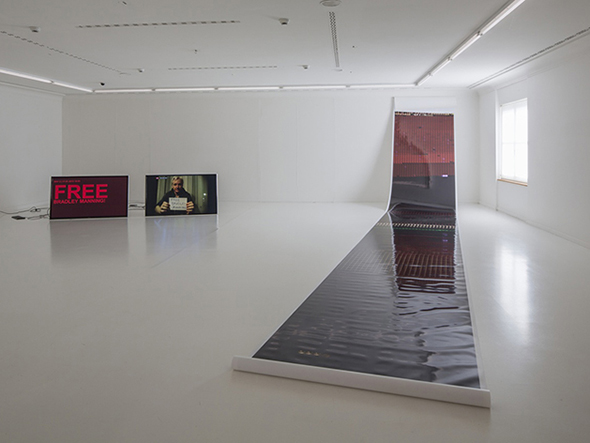
\includegraphics[width=0.65\textwidth]{bitnik_assange_installation_1}
	\caption{!Mediengruppe Bitnik, Ein Paket für Herrn Assange, 2014, Helmhaus Zürich, Installationsansicht, Fotografie 2014 (\url{https://wwwwwwwwwwwwwwwwwwwwww.bitnik.org/media/news/exhbition_helmhaus/thumb/bitnik_helmhaus_028_1600_1280.jpg}, 17.02.2015).}
	\label{fig:bitnik_assange_installation_1}
\end{figure}

\begin{figure}[H]
	\centering
	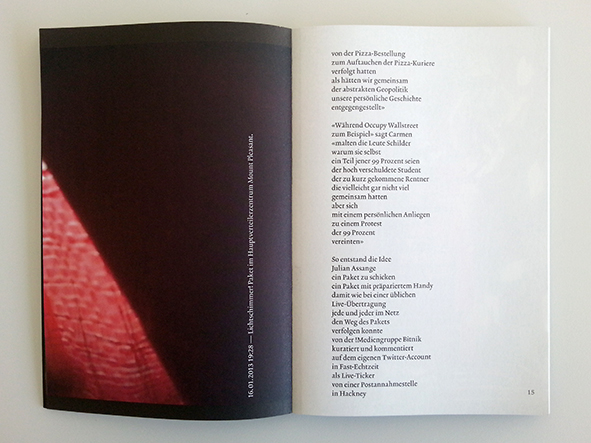
\includegraphics[width=0.65\textwidth]{bitnik_assange_catalog_1}
	\caption{!Mediengruppe Bitnik, Ein Paket für Herrn Assange, 2014, Helmhaus Zürich, Fotografie des Katalogs zur Ausstellung (\cite[14-15]{Ryser/MediengruppeBitnik:2014}).}
	\label{fig:bitnik_assange_catalog_1}
\end{figure}

\begin{figure}[H]
	\centering
	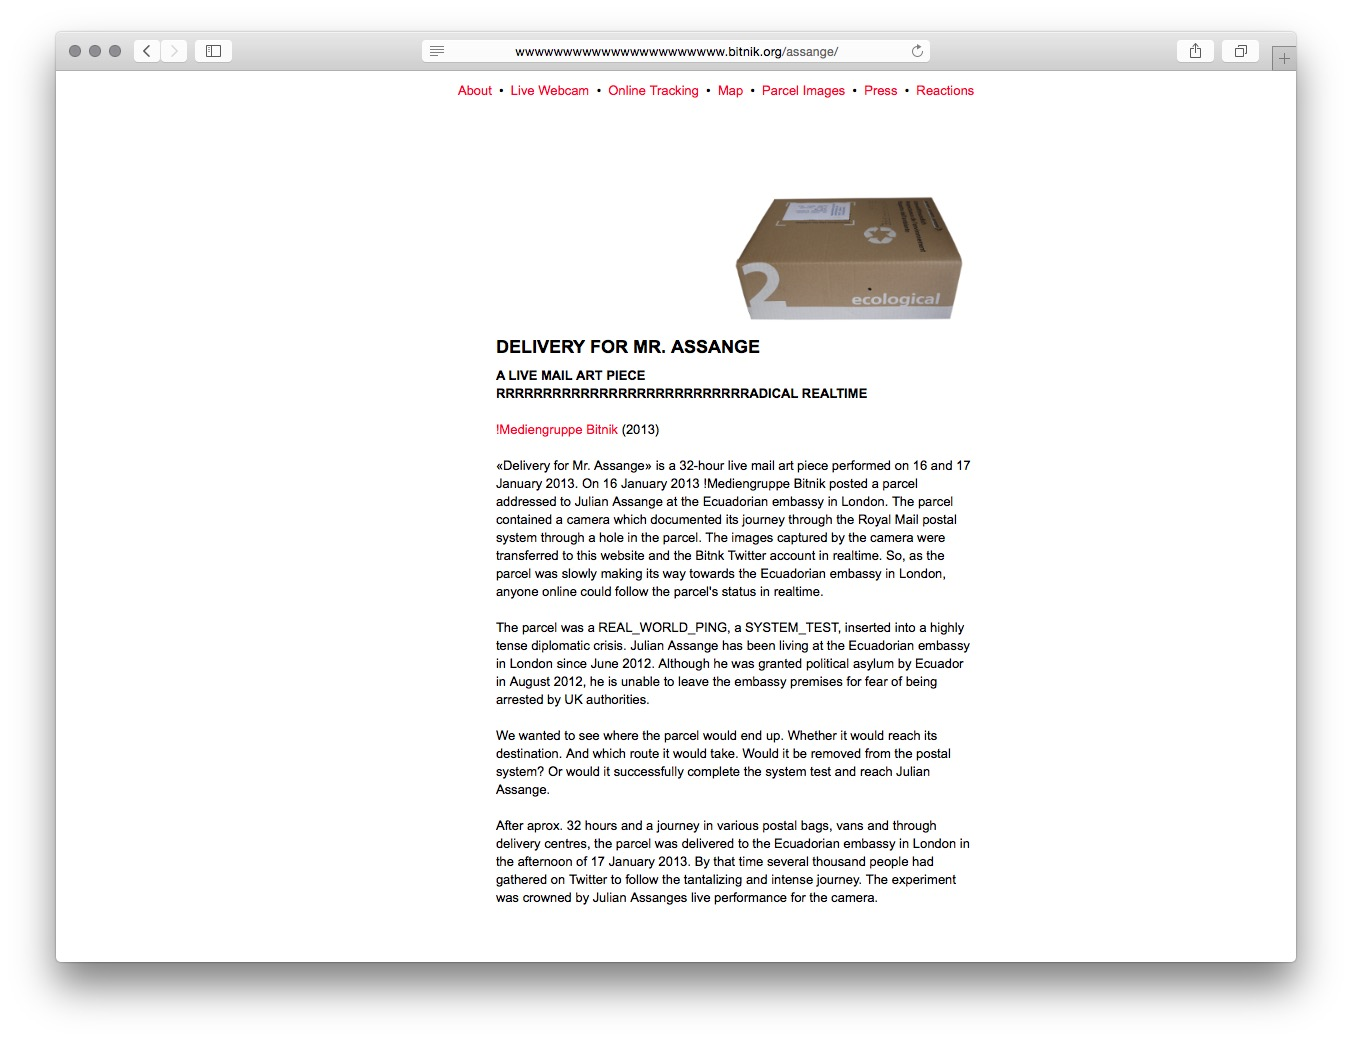
\includegraphics[width=0.65\textwidth]{bitnik_assange_website_1}
	\caption{!Mediengruppe Bitnik, Ein Paket für Herrn Assange, 2014, Screenshot der Webseite zum Werk  (\url{https://wwwwwwwwwwwwwwwwwwwwww.bitnik.org/assange/}, 17.02.2015).}
	\label{fig:bitnik_assange_Webseite_1}
\end{figure}

\begin{figure}[H]
	\centering
	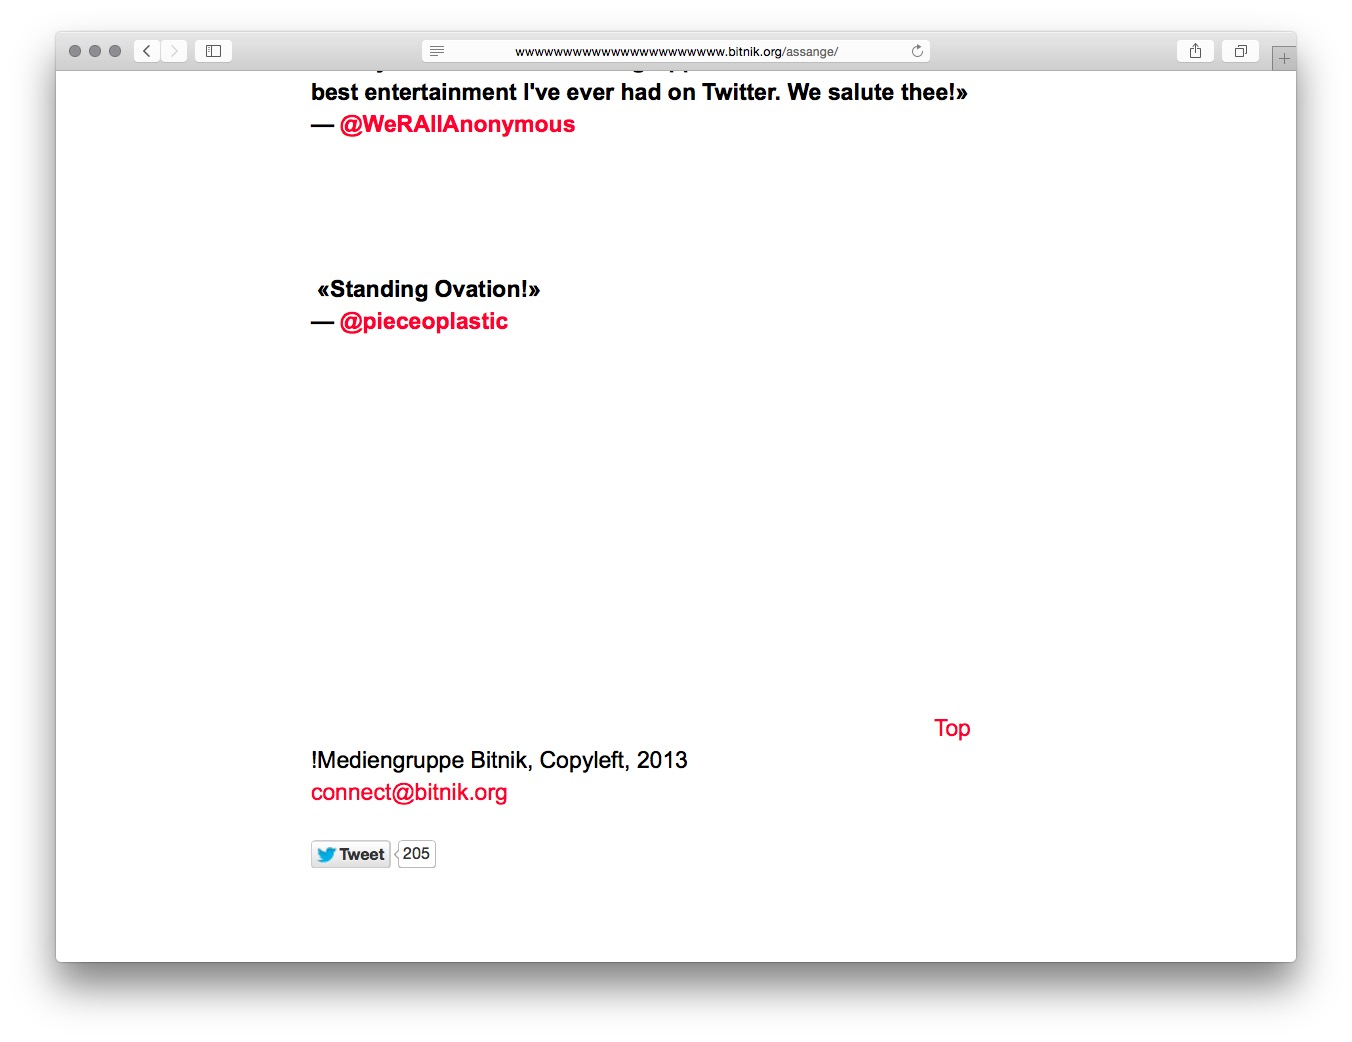
\includegraphics[width=0.65\textwidth]{bitnik_assange_website_2}
	\caption{!Mediengruppe Bitnik, Ein Paket für Herrn Assange, 2014, Detailaufnahme der Webseite zum Werk, Screenshot (\url{https://wwwwwwwwwwwwwwwwwwwwww.bitnik.org/assange/}, 17.02.2015).}
	\label{fig:bitnik_assange_Webseite_2}
\end{figure}

\begin{figure}[H]
	\centering
	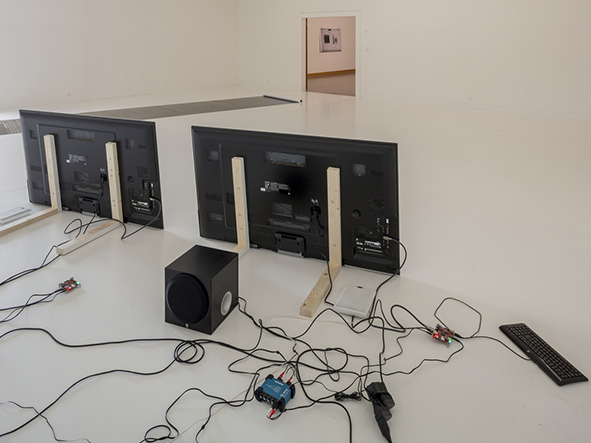
\includegraphics[width=0.65\textwidth]{bitnik_assange_installation_2}
	\caption{!Mediengruppe Bitnik, Ein Paket für Herrn Assange, 2014, Helmhaus Zürich, Cubieboard links neben der Tastatur, Fotografie 2014 (\url{https://wwwwwwwwwwwwwwwwwwwwww.bitnik.org/media/news/exhbition_helmhaus/thumb/bitnik_helmhaus_034_1600_1280.jpg}, 17.02.2015).}
	\label{fig:bitnik_assange_installation_2}
\end{figure}

% Waldvogel
\begin{figure}[H]
	\centering
	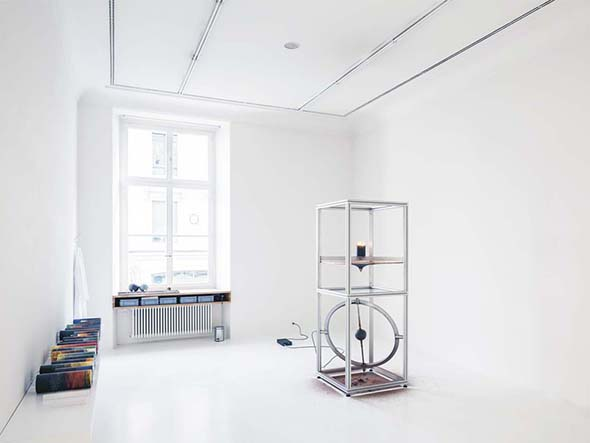
\includegraphics[width=0.65\textwidth]{waldvogel_rppm_installation_1}
	\caption{Christian Waldvogel, Random Planet Production Machine, 2014, Helmhaus Zürich, Installationsansicht, Fotografie 2014 (\url{http://waldvogel.com/cms/files/projects/helmhaus-zuerich/helmhaus_0005_MBCW.jpg}, 17.02.2015).}
	\label{fig:waldvogel_rppm_installation_1}
\end{figure}

\begin{figure}[H]
	\centering
	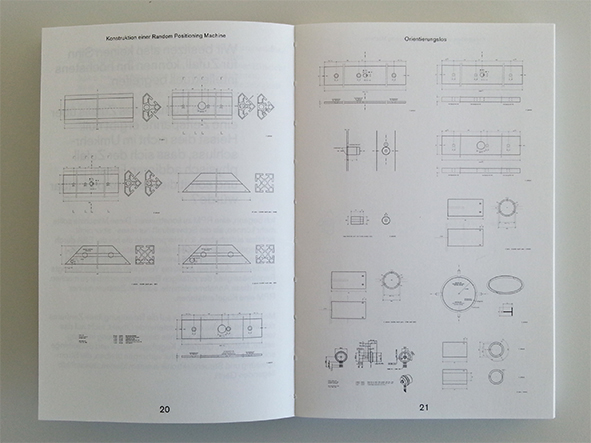
\includegraphics[width=0.65\textwidth]{waldvogel_rppm_catalog_1}
	\caption{Christian Waldvogel, Random Planet Production Machine, 2014, Helmhaus Zürich, Baupläne der RPPM, Fotografie des Katalogs zur Ausstellung (\cite[20-21]{Waldvogel:2014}).}
	\label{fig:waldvogel_rppm_catalog_1}
\end{figure}

\begin{figure}[H]
	\centering
	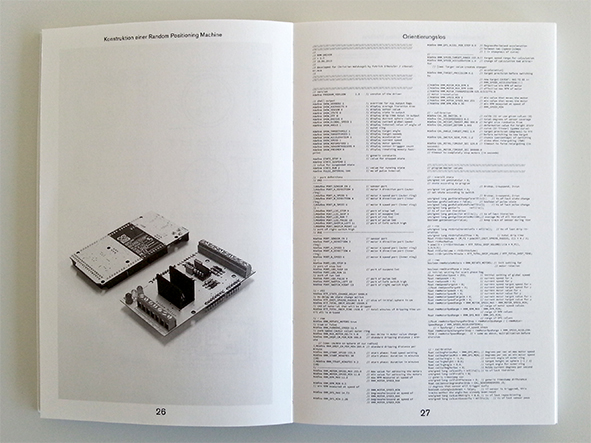
\includegraphics[width=0.65\textwidth]{waldvogel_rppm_catalog_2}
	\caption{Christian Waldvogel, Random Planet Production Machine, 2014, Helmhaus Zürich, Links die Leiterplatte, rechts ein Ausschnitt des Quellcodes der Steuerungssoftware, Fotografie des Katalogs zur Ausstellung (\cite[26-27]{Waldvogel:2014}).}
	\label{fig:waldvogel_rppm_catalog_2}
\end{figure}

\begin{figure}[H]
	\centering
	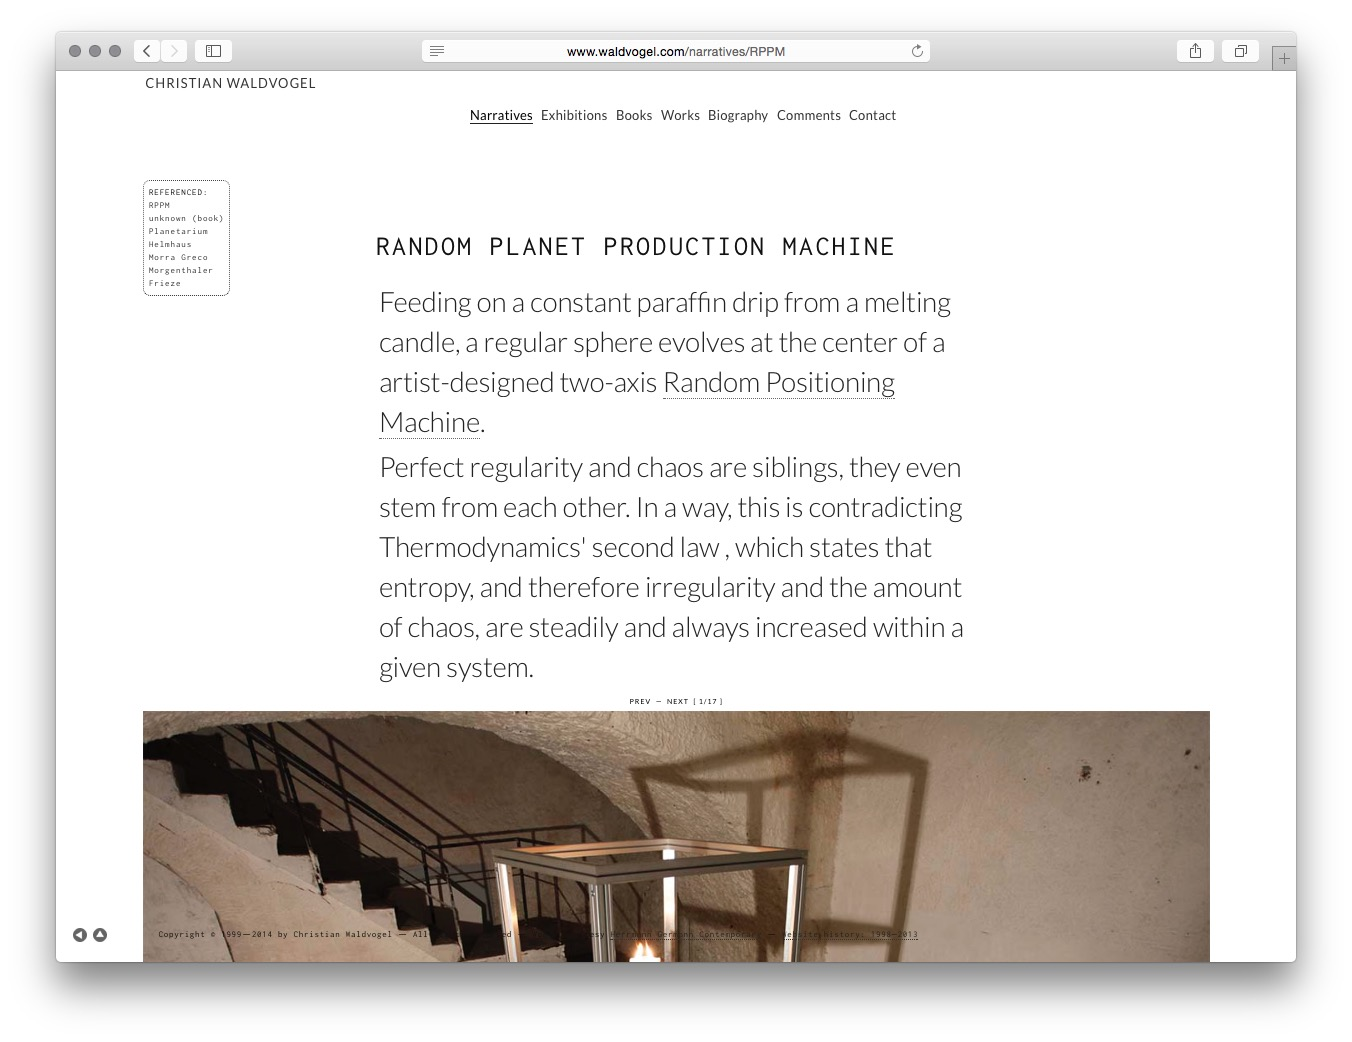
\includegraphics[width=0.65\textwidth]{waldvogel_rppm_website_1}
	\caption{Christian Waldvogel, Random Planet Production Machine, 2014, Screenshot der Webseite zum Werk (\url{http://www.waldvogel.com/narratives/RPPM}, 17.02.2015).}
	\label{fig:waldvogel_rppm_Webseite_1}
\end{figure}

% Levin
\begin{figure}[H]
	\centering
	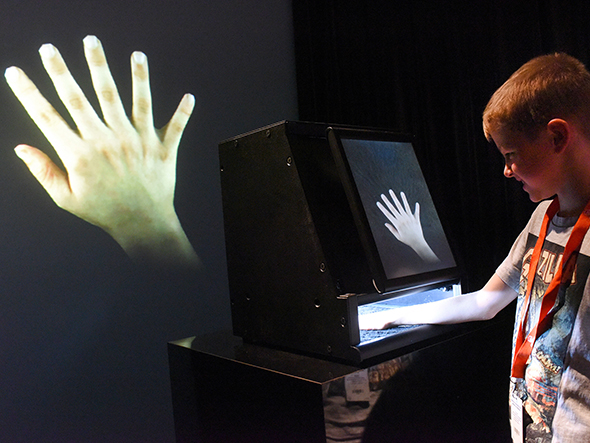
\includegraphics[width=0.7\textwidth]{levin_hands_installation_1}
	\caption{Golan Levin, Augmented Hand Series, 2014, Installationsansicht, Fotografie 2014 (\url{http://www.flong.com/storage/images/projects/augmented-hand-series.jpg}, 17.02.2015).}
	\label{fig:levin_hands_installation_1}
\end{figure}

\begin{figure}[H]
	\centering
	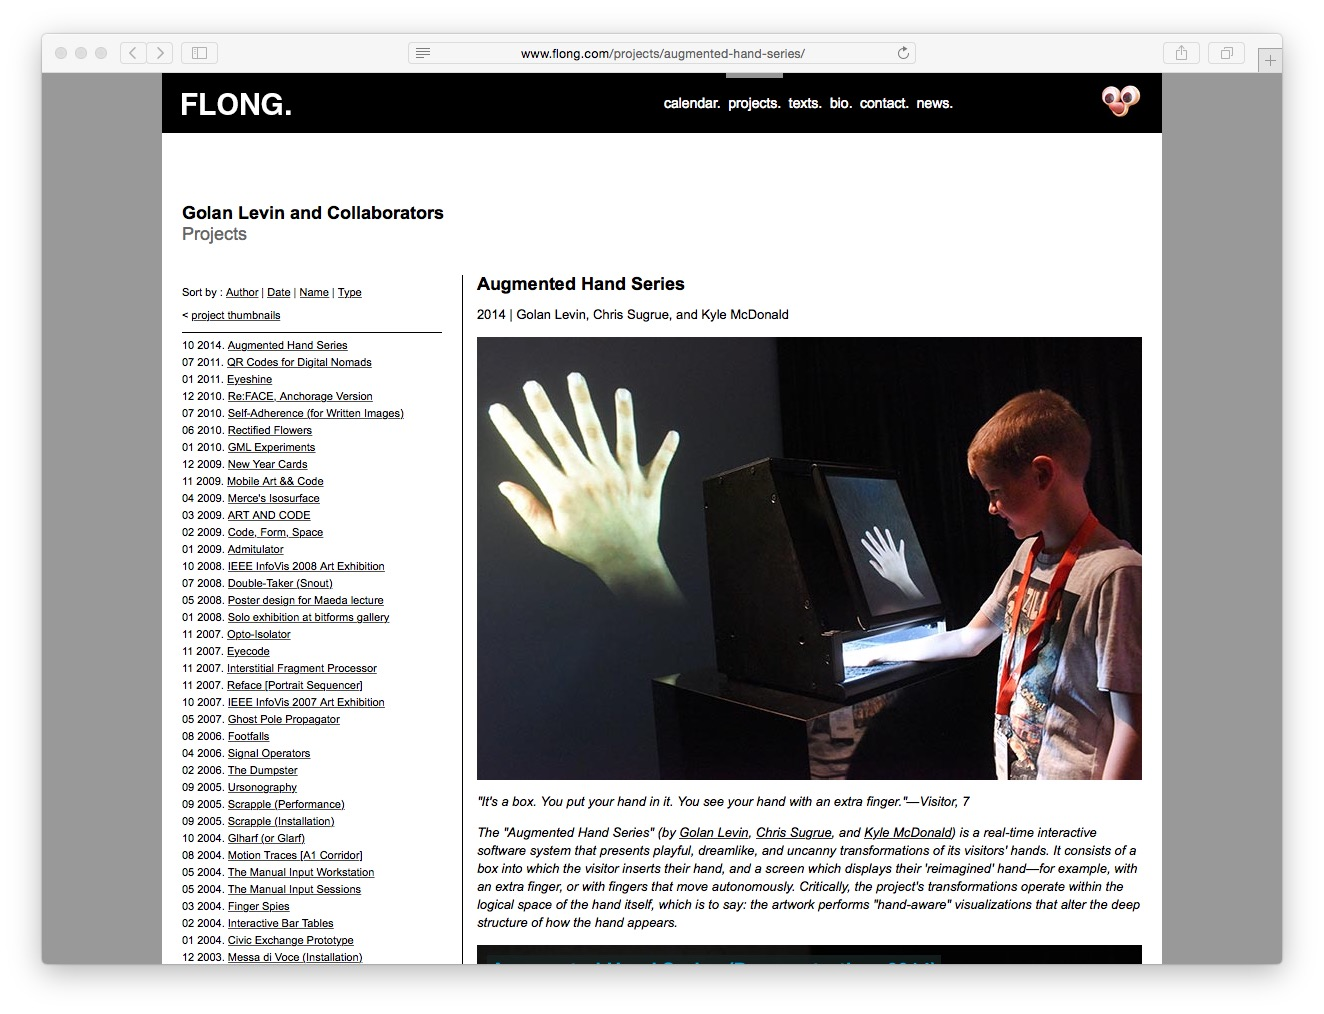
\includegraphics[width=0.7\textwidth]{levin_hands_website_1}
	\caption{Golan Levin, Augmented Hand Series, 2014, Details Aufnahme der Webseite zum Werk, Screenshot  (\url{http://www.flong.com/projects/augmented-hand-series/}, 17.02.2015).}
	\label{fig:levin_hands_Webseite_1}
\end{figure}


% ---
\part*{Anhang}

\phantomsection
\addcontentsline{toc}{chapter}{Anhang:Einige Open Source Projekte}
\chapter*{Einige Open Source Projekte}

Nachfolgend die Liste der in der Einleitung erwähnten Open Source Projekte. Die Reihenfolge entspricht derjenigen der Aufzählung. Die Auswahl der Projekte ist zufällig und nicht repräsentativ. Links zuletzt aufgerufen am 10.12.2014.

\begin{itemize}
	\item Framework: Twitter Bootstrap (\url{http://getbootstrap.com/})
	\item Webbrowser: Chromium (\url{http://www.chromium.org/})
	\item Betriebssystem: Lubuntu Linux (\url{http://lubuntu.net/})
	\item Mikrocontroller: Arduino (\url{http://www.arduino.cc/})
	\item Programmierumgebung: Arduino IDE (\url{http://www.arduino.cc/} basierend auf Processing \url{http://processing.org/})
	\item Computer System: Raspberry Pi (\url{http://www.raspberrypi.org/})
	\item Strickautomaten: OpenKnit \url{http://openknit.org/build/}
	\item 3D-Drucker: RepRap (\url{http://reprap.org/})
	\item Lexika: Wikipedia (\url{http://wikipedia.org})
	\item Handprothesen: Open Hand Project (\url{http://www.openhandproject.org/})
	\item Humanoide Roboter: Poppy Humanoid (\url{https://www.poppy-project.org/creatures/poppy-humanoid/})
	\item Video Games: Sintel the Game (\url{http://sintelgame.org/})
	\item Gamekonsolen: OUYA (\url{https://www.ouya.tv/})
	\item CNC-Fräsmaschinen: Shapeoko (\url{http://www.shapeoko.com/})
	\item Häuser: Wiki House (\url{http://www.wikihouse.cc/})
	\item Möbelstücke: z.B. der Sketch Chair (\url{http://www.sketchchair.cc/)})
	\item Zeichensätze: Die Openfont Library  (\url{http://openfontlibrary.org/})
	\item Sciencefiction Novelle: Die Triologie von Stephen J. Sweeney \emph{The Battle for the Solar System} (\url{http://www.battleforthesolarsystem.com/downloads/#knightsFirst})
	\item Bier: Free Beer (\url{http://freebeer.org/blog/})
	\item Pop-Musik: Das Album \emph{Pulse of the Earth} von Hungry Lucy (\url{http://music.hungrylucy.com/album/pulse-of-the-earth})
	\item Comic Strip: Mimi and Deunice (\url{http://mimiandeunice.com/})
	\item Animationsfilm: Sita sings the blues (\url{http://www.sitasingstheblues.com/})
	\item Spielfilm: Valkaama (\url{http://www.valkaama.com/})
	\item Filmfestival: Das Barcelona Creative Commons Film Festival das 2010 erstmals unter dem Slogan \emph{Copy this Festival} stattfand, erfreut sich seither jährlich steigender Besucherzahlen.
	\item Galerie: Open Source Galery in Brooklyn USA (\url{http://open-source-gallery.org/})
\end{itemize}

\end{document}
